%% LaTeX Beamer presentation template (requires beamer package)
%% see http://bitbucket.org/rivanvx/beamer/wiki/Home
%% idea contributed by H. Turgut Uyar
%% template based on a template by Till Tantau
%% this template is still evolving - it might differ in future releases!


\documentclass{beamer}
 
\mode<presentation>
{
\usetheme{NYU}

\setbeamercovered{transparent}
}

\usepackage[english]{babel}
\usepackage[latin1]{inputenc}

% font definitions, try \usepackage{ae} instead of the following
% three lines if you don't like this look
\usepackage{mathptmx}
\usepackage[scaled=.90]{helvet}
\usepackage{courier}


\usepackage[T1]{fontenc}


\usepackage{comment}
%usepackage{appendixnumberbeamer}
%\usepackage{amsmath}
\usepackage{pgfpages}
\usepackage{float}
% citations
\usepackage{natbib}
\usepackage{lipsum}
\usepackage[export]{adjustbox}

\bibpunct{(}{)}{;}{a}{,}{,}
\def\citeapos#1{\citeauthor{#1}'s (\citeyear{#1})}
\renewcommand{\bibsection}{\subsubsection*{\bibname } }

\title{Modelling Federal Open Market Committee Decisions Using ML and NLP}

%\subtitle{}

% - Use the \inst{?} command only if the authors have different
%   affiliation.
%\author{F.~Author\inst{1} \and S.~Another\inst{2}}
\author{Jeremy Lao \& John Reynolds} 

% - Use the \inst command only if there are several affiliations.
% - Keep it simple, no one is interested in your street address.
\institute[NYU]
{
Department of Computer Science\\
Courant Institute of Mathematical Sciences, NYU\\
  \texttt{}
}

\date{Date}


% This is only inserted into the PDF information catalog. Can be left
% out.
\subject{Subject}



% If you have a file called "university-logo-filename.xxx", where xxx
% is a graphic format that can be processed by latex or pdflatex,
% resp., then you can add a logo as follows:

\pgfdeclareimage[height=0.5cm]{university-logo}{nyu_long_color}
\logo{\pgfuseimage{university-logo}}




% If you wish to uncover everything in a step-wise fashion, uncomment
% the following command:

%\beamerdefaultoverlayspecification{<+->}

\begin{document}

\begin{frame}
\titlepage
\end{frame}



\begin{frame}
Federal Open Market Committee (FOMC): Maximum Employment, Stable Inflation, Financial Stability
\vspace{-3mm}
\begin{figure}[H]
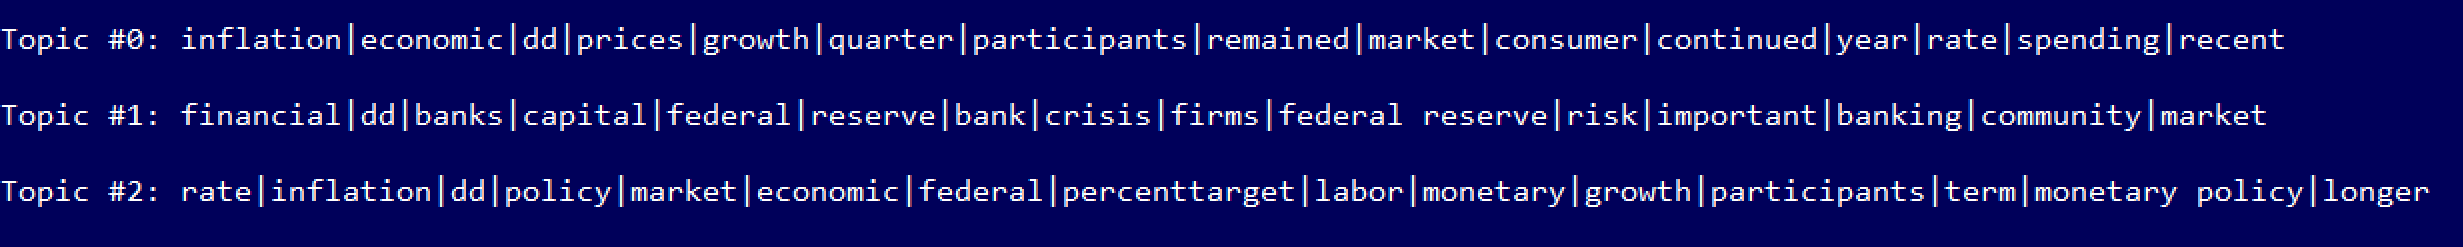
\includegraphics[width=1\textwidth]{../output/data_for_graphs/Topic-Model-3-topics.PNG}
\end{figure}
\vspace{-5mm}

Ngrams (unigrams to 10-grams) - F1 Score
\vspace{-1mm}
\begin{figure}[H]
\begin{center}
\includegraphics[width=.25\textwidth]{"../output/data_for_graphs/log_lasso_f1".pdf}
\includegraphics[width=.25\textwidth]{"../output/data_for_graphs/naive_bayes_f1".pdf}
\end{center}
\end{figure}
\vspace{-5mm}

Reduced Features (stacked documents, larger Ngrams) - F1 Score
\vspace{-1mm}
\begin{figure}[H]
\includegraphics[width=.22\textwidth]{"../output/data_for_graphs/nn_40_40_f1_stacked".pdf}
\includegraphics[width=.22\textwidth]{"../output/data_for_graphs/nn_40_f1_stacked".pdf}
\includegraphics[width=.22\textwidth]{"../output/data_for_graphs/log_lasso_f1_stacked".pdf}
\includegraphics[width=.22\textwidth]{"../output/data_for_graphs/naive_bayes_f1_stacked".pdf}
\end{figure}

\end{frame}


\end{document}
